%%
%% Copyright 2007-2020 Elsevier Ltd
%%
%% This file is part of the 'Elsarticle Bundle'.
%% ---------------------------------------------
%%
%% It may be distributed under the conditions of the LaTeX Project Public
%% License, either version 1.2 of this license or (at your option) any
%% later version.  The latest version of this license is in
%%    http://www.latex-project.org/lppl.txt
%% and version 1.2 or later is part of all distributions of LaTeX
%% version 1999/12/01 or later.
%%
%% The list of all files belonging to the 'Elsarticle Bundle' is
%% given in the file `manifest.txt'.
%%
%% Template article for Elsevier's document class `elsarticle'
%% with harvard style bibliographic references

%\documentclass[preprint,12pt,authoryear]{elsarticle}

%% Use the option review to obtain double line spacing
%% \documentclass[authoryear,preprint,review,12pt]{elsarticle}

%% Use the options 1p,twocolumn; 3p; 3p,twocolumn; 5p; or 5p,twocolumn
%% for a journal layout:
%% \documentclass[final,1p,times,authoryear]{elsarticle}
%% \documentclass[final,1p,times,twocolumn,authoryear]{elsarticle}
%% \documentclass[final,3p,times,authoryear]{elsarticle}
%% \documentclass[final,3p,times,twocolumn,authoryear]{elsarticle}
%% \documentclass[final,5p,times,authoryear]{elsarticle}
 \documentclass[final,5p,times,twocolumn,authoryear]{elsarticle}

%% For including figures, graphicx.sty has been loaded in
%% elsarticle.cls. If you prefer to use the old commands
%% please give \usepackage{epsfig}

%% The amssymb package provides various useful mathematical symbols
\usepackage{amssymb}
\usepackage{caption}
\usepackage{hyperref}

%% Hide "preprint submitted by" line
\makeatletter
\def\ps@pprintTitle{%
  \let\@oddhead\@empty
  \let\@evenhead\@empty
  \let\@oddfoot\@empty
  \let\@evenfoot\@oddfoot
}
\makeatother
%% The amsthm package provides extended theorem environments
%% \usepackage{amsthm}

%% The lineno packages adds line numbers. Start line numbering with
%% \begin{linenumbers}, end it with \end{linenumbers}. Or switch it on
%% for the whole article with \linenumbers.
%% \usepackage{lineno}

%% You might want to define your own abbreviated commands for common used terms, e.g.:
\newcommand{\kms}{km\,s$^{-1}$}
\newcommand{\msun}{$M_\odot}

\begin{document}


\begin{frontmatter}

%% Title, authors and addresses

%% use the tnoteref command within \title for footnotes;
%% use the tnotetext command for theassociated footnote;
%% use the fnref command within \author or \affiliation for footnotes;
%% use the fntext command for theassociated footnote;
%% use the corref command within \author for corresponding author footnotes;
%% use the cortext command for theassociated footnote;
%% use the ead command for the email address,
%% and the form \ead[url] for the home page:
%% \title{Title\tnoteref{label1}}
%% \tnotetext[label1]{}
%% \author{Name\corref{cor1}\fnref{label2}}
%% \ead{email address}
%% \ead[url]{home page}
%% \fntext[label2]{}
%% \cortext[cor1]{}
%% \affiliation{organization={},
%%            addressline={},
%%            city={},
%%            postcode={},
%%            state={},
%%            country={}}
%% \fntext[label3]{}

\title{%
High-Throughput Phenotyping of Populus Trichocarpa Using Computer Vision \\
\large SMC Data Challenge \#1
}

%% use optional labels to link authors explicitly to addresses:
%% \author[label1,label2]{}
%% \affiliation[label1]{organization={},
%%             addressline={},
%%             city={},
%%             postcode={},
%%             state={},
%%             country={}}
%%
%% \affiliation[label2]{organization={},
%%             addressline={},
%%             city={},
%%             postcode={},
%%             state={},
%%             country={}}

\author[]{Vivaan Singhvi}
\author[]{Langalibelele Lunga}
\author[]{Pragya Nidhi}
\author[]{Chris Keum}
\author[]{Varrun Prakash}

\begin{abstract}
%% Text of abstract
	High-throughput phenotyping refers to the non-destructive and efficient evaluation of plant phenotypes. Machine Learning methods offer the prospect of addressing two major challenges in phenotyping plants: efficiency in handling large datasets and extraction of specific traits. Previous techniques, such as the application of Deep Neural Nets in tandem with automated cameras, to our best knowledge, refrain from using physically labeled plants to organize datasets. To accomplish this, we used Optical Character Recognition(OCR) to read the physical labels on the plants, image segmentation techniques(OpenCv, FacebookSAM)  in order to apply Machine Learning algorithms(RandomForestClassifier, XGradientBoosting) for plant morphology classifications, and analyzed encoded EXIF tag information for the purpose of finding correlations between phenotypes. We used a  Populus Trichocarpa  plant dataset provided by Oak Ridge National Laboratory, with 1,672 image files of plants labeled with treatment( Control or Drought), block, row, position, and genotype. We found that OCR techniques, such as PaddleOCR, successfully read 91.3\% of the labeled plants, allowing for labeled information to be accurately placed in a pandas Dataframe. The success of the OCR carried into our XGradientBoosting and RandomForestClassifier techniques, which classified leaf morpholgoies by leaf shape and color with an accuracy of 62.82\%. Finally, we found [insert findings from step 4]. The use of Machine Learning in High-throughoutPut Phenotyping has shown to be effective in analyzing large plant datasets[Improve this sentence]. It allows for efficient and environmentally friendly classification of plants.
\end{abstract}

%%Graphical abstract
%\begin{graphicalabstract}
%\includegraphics{grabs}
%\end{graphicalabstract}

%%Research highlights
%\begin{highlights}
%\item Research highlight 1
%\item Research highlight 2
%\end{highlights}

\begin{keyword}
%% keywords here, in the form: keyword \sep keyword, up to a maximum of 6 keywords
computer vision \sep machine learning \sep high-throughput phenotyping

%% PACS codes here, in the form: \PACS code \sep code

%% MSC codes here, in the form: \MSC code \sep code
%% or \MSC[2008] code \sep code (2000 is the default)

\end{keyword}


\end{frontmatter}

%\tableofcontents

%% \linenumbers

%% main text

\section{Introduction}
\label{intro}

Image-based phenotyping refers to a breakthrough technology used in plant biology and agriculture to examine and assess plants’ “anatomical, ontological, physiological, and biochemical features” through the use of images. Previous studies have shown its potential as a noninvasive replacement for traditional on field techniques used to extract important phenotypic data. In recent years, this potential has been further intensified by coupling image-based phenotyping techniques with machine learning algorithms. This new approach, called high throughput phenotyping, has enabled the extraction of phenotypes from “complex” plant image datasets that were previously challenging to analyze efficiently. Furthermore, more recent studies have shown that the technology holds potential in identifying correlations between phenotype, genotype, and environmental metadata. 

In this study, we aim to develop an accurate Machine Learning Model for High Throughput Phenotyping of leaves’ morphological traits (e.g. leaf size, shape, color) in plant images; unlike datasets in previous research, the dataset used in this study contains physical labels within the images, each containing important information on treatment (Control or Drought), block, row, position, and genotype. As a result, this study will deal with a new aspect of image-based phenotyping namely, extracting data from the white labels to identify correlations between leaves’ phenotypes and data embedded within the white labels. Given this information, the study aims to answer the following questions: 

\begin{enumerate}

\item Is it possible to use optical character recognition (OCR) or machine learning techniques to “Read” the label on each tag and generate a spreadsheet containing the treatment, block, row, position, and genotype? Doing this would dramatically simplify data collection, as this information is usually collected manually.

\item Can machine learning differentiate and classify different leaf morphologies among genotypes by classifying leaf shape or color characteristics?

\item Can a predictive model be built using leaf morphology classifications that may indicate that a particular genotype was cultivated in a “drought” or “control” condition?

\item GPS and other camera information are encoded in EXIF tags. Can this data be used to determine characteristics such as leaf size? Can other data, such as soil maps, weather, etc. be used to find correlations among phenotypes?

\end{enumerate}

\section{Related Works}
\label{related_works}

Traditionally, plant morphologies would have to be analyzed by hand, wasting time and potentially damaging the environment. Now, with breakthroughs in high throughput image phenotyping led by Machine Learning techniques, methods such as Automated Machine Learning \citep{koh2021automated}, Computer Vision with Deep Learning \citep{mochida2019computer},  and Convolutional Neural Networks(CNNs) \citep{pound2017deep}, have allowed for efficient and timely analysis of plant phenotypes. With these methods, researchers are able to extract features from plants and classify plant morphologies effectively with little effect on the plant environment.

\subsection{Advancements in High Throughput Phenotyping Techniques}
\label{related_works_1}

Advancements in the field of plant phenotyping have been pioneered by technology. 
From using hardware, such as Raspberry Pi imaging systems \citep{tausen2020greenotyper} to thermographical sensing techniques \citep{walter2015plant}, research in the field of high phenotyping has led to an acceleration in working efficiency. Plants are now able to be analyzed in fast, effective, and accurate methods allowing for plant to be used in scientific discoveries. In our study, we rely on machine learning techniques to classify morphologies based on a phone image dataset provided.

\subsection{Machine Learning Approaches for Phenotypic Analysis}
\label{related_works_2}

Machine Learning has enabled researchers with computer vision, allowing them to create programs that “read” image information in real time. In addition, it increases the efficiency of obtaining leaf morphology data. However, researchers have found that the use of traditional classification techniques, such as RandomForrestClassifier, have a high performance, but do not generalize well across datasets \citep{pound2017deep}. In order to increase accuracy of models and the generalization of the model, Deep Learning techniques have been introduced. With deep learning models, models train themselves iteratively until they reach a desired outcome. These techniques, such as Convolutional Neural Networks \citep{koh2021automated, pound2017deep} have shown to be highly accurate in classifying plant structures while maintaining performance across different datasets. Convolutional Networks consist of several layers, which allow for more discriminative and detailed analysis of the plant image, leading to highly accurate classifications. In our study, we use traditional methods(GradientBoosting, RandomForest) to classify plant morphology, as our focus is on organizing the plant images into an easily readable dataset and performing classifications, instead of creating models highly transferable across datasets.

\subsection{Applications of High Throughput Phenotyping with Machine Learning}
\label{related_works_3}

Due to global events, such as climate change and global population increase, the ability to produce large amounts of healthy food will be crucial to society. With Machine Learning being used for phenotyping, researchers will be able to rapidly analyze food crops to maximize production and crop breeding \citep{arya2022deep, shakoor2017high}.
As climate change and global population increases, global crop yield will have to increase to provide for the growing populations. Further research has shown that climate change will continue to negatively affect crops and cause crop diseases \citep{newton2011implications}, hence the need for effective and precise analysis of plants, which is done with Machine Learning models. In our study, we aim to show how Machine Learning can be used to organize plant data, dissect plant images into meaningful classifications, and allow for rapid investigation of plants for scientists in the field of plant phenotyping.

\section{Methodology}
\label{method}
%%\label{}

Given the nature of the project, there are many aspects requiring obtaining large files, such as the dataset itself or large models. Therefore, all scripts needed to fully set up the project (downloading large files or setting up a large virtual environment), are viewable in the \verb|scripts/| folder in the GitHub repository, linked in Section \ref{code}.

All solutions to the challenge were implemented in Python 3.9/3.10. Several notable libraries used throughout the project include: OpenCV \citep{opencv_library}, the open-source computer vision library; Scikit-Learn \citep{scikit-learn}, Python implementations of dozens of machine learning algorithms and data processing tools; Pandas \citep{mckinney2010data}, a data manipulation library featuring the powerful \verb|DataFrame| object; and NumPy \citep{harris2020array}, an array manipulation library crucial for fast operations on images.

\subsection{Reading Labels with Optical Character Recognition}
\label{step_1}

To read the text, a pre-trained Optical Character Recognition (OCR) model seemed like the optimal choice. However, there are several models high-performing models available for use. The three candidates chosen for this project were \verb|PyTesseract| \citep{lee2017pytesseract}, \verb|EasyOCR| \citep{jaided2020easyocr}, and \verb|PaddleOCR| \citep{du2020ppocr}.

The three models were tested using metrics of performance and efficiency, which were measured through their accuracy score and time taken on a sample dataset of nine images. The results of the testing can be viewed in \ref{app_ocr_testing}.

\verb|PaddleOCR| was superior in speed, being significantly faster than \verb|EasyOCR| and marginally faster than \verb|PyTesseract|. It is also more accurate in both measurements, having a higher accuracy score with and without null values.

In order to fix the aforementioned null values from the OCRs, images went through augmentation, with subsequent attempts being made to read text during each step. First, images are rotated 45 degrees in order to fix potential orientation issues. Then, the original image is thresholded using OpenCV's \verb|adaptiveThreshold| to amplify the edges. Finally, if nothing works, the image is both rotated and thresholded.

\begin{center}
    \includegraphics[width=0.45\textwidth]{images/step1_pipeline.png}
    \captionof{figure}{Different versions of images tried for optical character recognition, in order}
\end{center}

After the text was read by the OCR, regular expressions (RegEx) were used to find the precise details mentioned in the dataset: treatment, block, row, position, and genotype. A subjective analysis of the images in the dataset showed that the treatment was either a ‘C’ or a ‘D’, and the remaining features followed the RegEx patterns below (note: \verb|\d| represents a digit, anything between 0-9) :

\begin{verbatim}
  Block:      B\d+
  Row:        R\d+
  Position:   P\d+
  Genotype:   [A-Z]{2,}(-\d+)+(_\d+)*(_[A-Z]+)?
\end{verbatim}

After all the text is read and processed, it is converted to a Pandas \verb|DataFrame| and saved to an Excel file.

\subsection{Classifying Leaf Morphologies with Image Processing}
\label{step_2}

In order to be able to determine the morphological characteristics of the plants, it is necessary to perfectly segment the leaves from each image. This proved to be a challenging endeavor due to the complexity of the background of the images, other datasets, such as the Komatsuna dataset, \citep{uchiyama2017easy} had 'cleaner' image backgrounds.

To obtain perfect masks for leaves in each image, the Segment Anything Model (SAM) \citep{kirillov2023segment} is the obvious choice. Being a relatively new and groundbreaking model, this paper is one of the first to utilize a pre-trained model of its caliber.

The \verb|AutomaticMaskGenerator| provided generates accurate masks for everything in an image. However, it has two issues: it may generate too many masks (especially for images as cluttered as those in the dataset), and is computationally expensive, taking too long to be a plausible approach for all 1672 images in this dataset. Through a \verb|SamPredictor| in conjunction with an ONNX \citep{bai2019onnx} \verb|InferenceSession|, masks would generate much quicker, and only from desired points. However, to obtain these desired points, the images would have to be processed to approximate the locations of the leaves.

The first step was to hide non-leaf elements in the image. A popular technique called HSV filtering was employed, used in a similar project by \cite{szachowicz2021komatsuna}. This involves filtering all pixels that are not between an HSV-encoded color range, helping eliminate many background objects such as wood, dirt, and of course, the label.

Then, OpenCV's implementation of the \verb|Canny| algorithm was used to highlight significant edges in the image, which were present around the boundary of leaves but were minimal inside of them. However, some leaves had boundary edges with gaps, causing most contours detected (using OpenCV's \verb|findContours|) to be sporadic. Therefore, the edges were dilated in multiple iterations by using a large kernel, causing the boundaries to be closed. After contours were found on the resulting image, they were filtered by pruning those that had a height or width (found using the \verb|boundingRect| function around each contour) too small compared to that of the image. Additionally, contours with not enough green inside them (namely less than $\frac{100}{255}$ green) were removed.

\begin{center}
	\centering
	\includegraphics[width=0.15\textwidth]{images/seg_pipeline/1.png}	
        \includegraphics[width=0.15\textwidth]{images/seg_pipeline/2.png}      	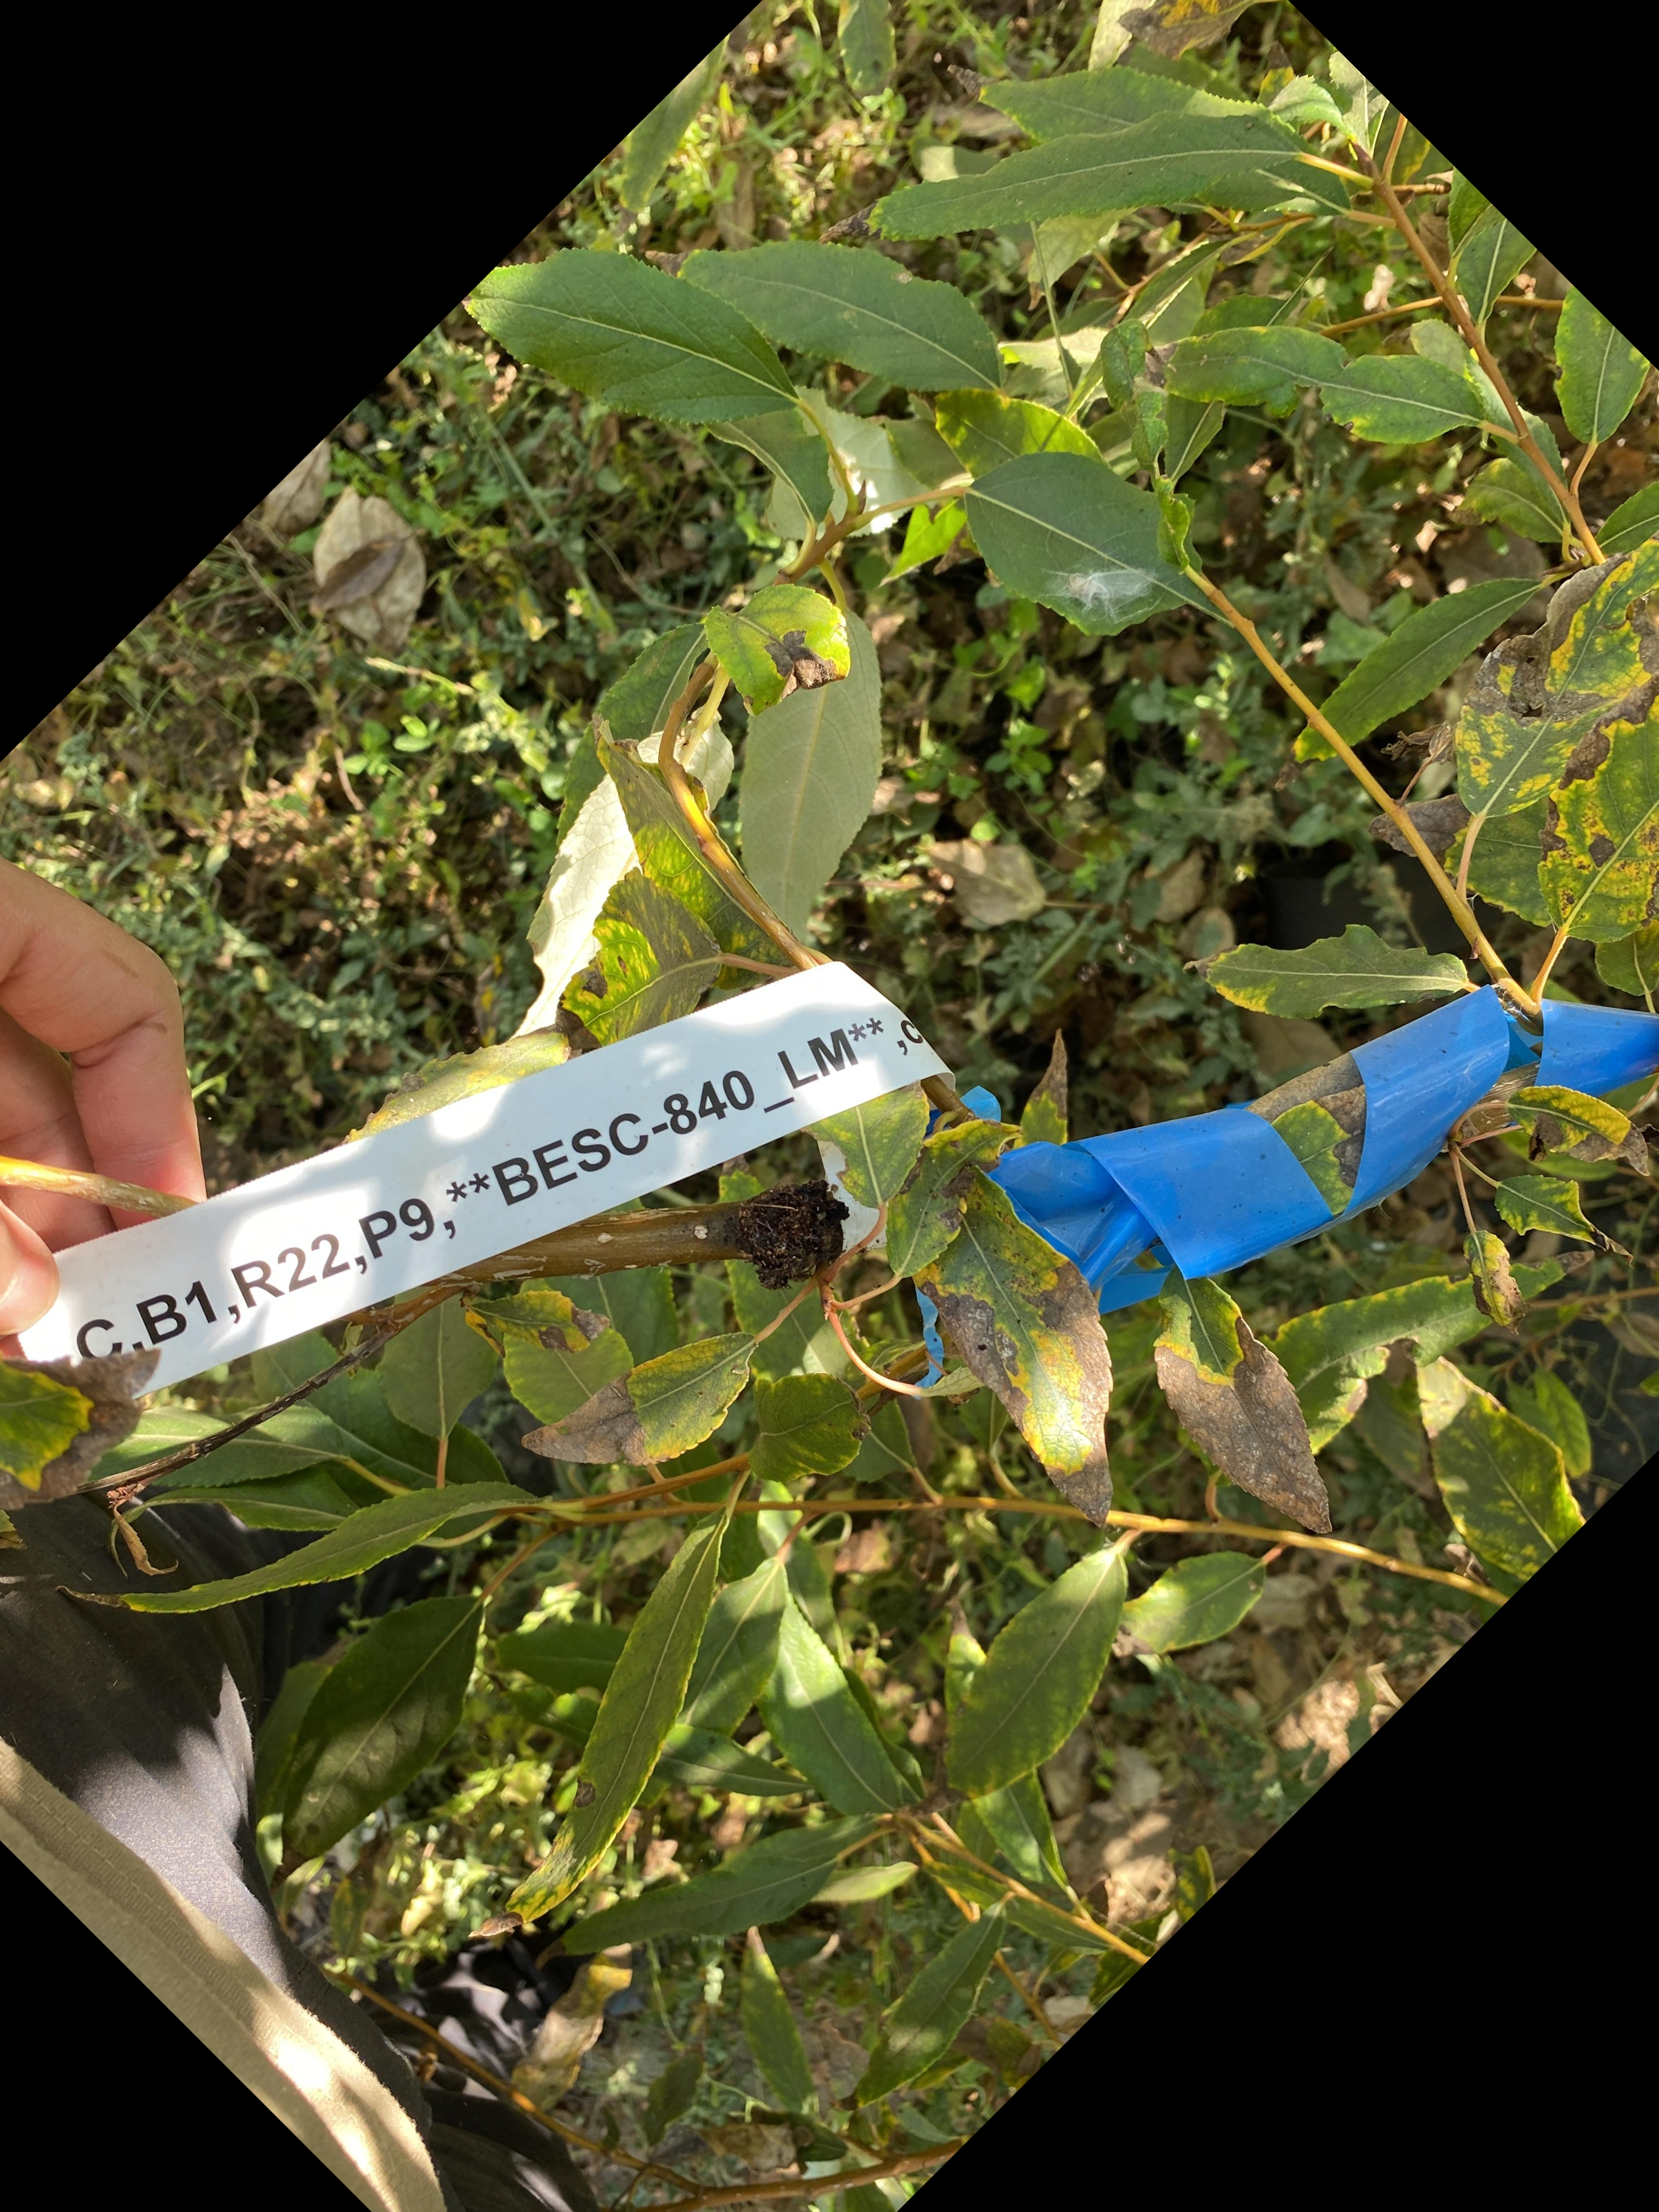
\includegraphics[width=0.15\textwidth]{images/seg_pipeline/3.png}	
	\includegraphics[width=0.15\textwidth]{images/seg_pipeline/4.png}	
	\includegraphics[width=0.15\textwidth]{images/seg_pipeline/5.png}	
	\includegraphics[width=0.15\textwidth]{images/seg_pipeline/6.png}	
	\captionof{figure}{Pipeline of image transformations for leaf approximation, read left to right}
	% \label{fig_mom0}%
\end{center}

To find the approximate points of these leaf contours, the midpoint was calculated using this simple formula, with $x, y, w, h$ being the outputs of OpenCV's \verb|boundingRect| function:

\begin{equation}
    \mbox{midpoint} = (x + \frac{w}{2}, y + \frac{h}{2})
\end{equation}

By using these points as target points for the SAM/ONNX mask predictor, leaves could reliably be obtained from the image. Masks could then be saved for each image by converting each of an image's masks to a random uniform grayscale value and combining them all into an image. While very accurate, however, some leaves detected by the program were not appropriate for use in morphology analysis. For example, some leaves could be cut off by another object, or, in rare cases, be green wood misinterpreted as leaves.

Thus, it was necessary to train a machine learning model that was able to accurately detect these kinds of 'bad' leaves. Training data was generated by showing randomly selected leaves and getting human input regarding their suitability, extracting their features, and storing the data in a file. The model was implemented using Scikit-Learn's \verb|RandomForestClassifier|. The model had an accuracy of 90.91\% on testing data generated by Scikit-Learn's \verb|train_test_split|.

\begin{center}
	\centering
	\includegraphics[width=0.15\textwidth]{images/seg_pipeline/6.png}	
        \includegraphics[width=0.15\textwidth]{images/seg_filter/1.png}      	\includegraphics[width=0.15\textwidth]{images/seg_filter/2.png}	
	\captionof{figure}{The process for filtering segmentations through the model: from contour approximations to generated masks to filtered masks}
	% \label{fig_mom0}%
\end{center}

Then, each leaf could be cropped and rotated, which, when combined with masking every pixel outside the its border, effectively highlighted and isolated it for visual purposes. By repeating this process for each image in the dataset, random leaves could then be selected to generate data for training the morphological classification model.

By using a slightly modified version of the aforementioned feature extraction function in conjunction with human labeling of leaves regarding their shape, color, and level of brown splotches, a \verb|MultiOutputClassifier| was able to be implemented with Scikit-Learn. More specifically, the \verb|XGBoost| algorithm was used for each of the three predicted features in the \verb|MultiOutputClassifier|.

TO BE CONTINUED (REWRITING NOT FINISHED YET).

\subsection{Treatment Predictions using Morphological Classifications}
\label{step_3}

The task for this step was to build a model to predict if a leaf was grown in a control or drought environment, given morphological classifications from the previous step. 

The challenge for using classification data as features to train a model with is that they are categorical, rather than quantitative variables; thus, extra transformations must be done to properly represent the data.

To properly represent the classifications, the method of one-hot encoding (MAYBE FIND SOURCE SAYING ITS GOOD) was implemented using the Pandas \verb|get_dummies| method. This is a process in which a feature is split into multiple columns, with each row having a one if it matches the column or a zero if it doesn't. 

\begin{center}
\resizebox{\columnwidth}{!}{%
\begin{tabular}{c||c c c c} 
 \hline
 leaf\_color & light\_green & dark\_green & yellow\_green & yellow  \\
 \hline
 light\_green & 1 & 0 & 0 & 0 \\
 yellow\_green & 0 & 0 & 1 & 0 \\
 dark\_green & 0 & 1 & 0 & 0 \\ 
 light\_green & 1 & 0 & 0 & 0 \\
 yellow & 0 & 0 & 0 & 1 \\
 \hline
\end{tabular}
}
\captionof{table}{Example transformation of a column with one-hot encoding, with the original column on the left and the encoded columns on the right}
\label{Table1}
\end{center}

This process was done with the leaf color and shape variables. However, since the level of brown splotches is ordinal, it was assigned levels 0, 1, 2, and 3, corresponding to ‘none’, ‘low’, ‘medium,’ and ‘high.’ Now, with all the data numerical, it could be used to train and test the model.

\subsection{Using EXIF Data to Assess Leaf Size and Analyze Correlations Between Morphologies and Environments}
\label{step_4}

Firstly, we aimed to measure the size of a leaf through metadata, encoded in EXIF Tags, which are embedded within each of the images. These EXIF tags typically give important information about the images, including the type of camera utilized, the distance of the camera from a photo, and photo dimensions (in pixels). In order to initiate the extraction of such metadata from the images, a package called “exif” was used and gave a variety of retrieval options. 

Out of all the metadata extracted from the EXIF tags, the most notable pieces of information included ResolutionX/Y tags and focal length. Although these pieces of information are crucial in developing a mechanism to measure leaf size in the dataset, the information provided simply does not suffice in determining leaf size; we needed information such as how far the leaf was from the camera, information that was not given from EXIF tags alone. This lack of information rendered the metadata as inadequate for direct measurement of leaf size. 

Another approach we considered to measure leaf size included using the white labels, held up by the researcher in each image, as a known reference object. Although this method seemed promising, there were certain limitations in most images in the dataset that prevented a consistent measurement. Firstly, the white label in the image was often obstructed by the researcher’s hands, as shown in Figure 1. This obstruction would ultimately interfere with alignment of the white label, making the label unreliable as an object of reference. Another limitation to this method came from the fact that the labels were often tilted, not in the same plane as the leaves. The tilt of the labels caused inaccuracies in measurement and would lead to misrepresentation of the true length. Along with that, there was no way of finding out how far forward or behind the leaf was relative to the tag, meaning the method would result in an inaccurate representation of the leaf.

In the second part of challenge 4, we aimed to find correlation among phenotypes using geographical features including soil type and weather conditions. Using the EXIF tags, we were able to retrieve the coordinates where the image was taken. We noticed all of the images contained were taken in approximately the same area, meaning weather would be the same for all plants. Along with that, most soil map APIs contain information about the soil in an area, so it would be unable to distinguish miniscule changes in locations. For all other potential geographical changes, due to the close proximity all images are taken in, we were unable to find out if there were any correlations. Not only was the location the same, the images were taken in a short time frame, within a week. This gave us the same limitations as the close location had. 


\section{Results}
%%\label{}

\subsection{Reading Labels with Optical Character Recognition}
\label{step_1}

\subsection{Classifying Leaf Morphologies with Image Processing}
\label{step_2}

\subsection{Treatment Predictions using Morphological Classifications}
\label{step_3}

\subsection{Using EXIF Data to Assess Leaf Size and Analyze Correlations Between Morphologies and Environments}
\label{step_4}

Overall, the metadata embedded in these specific EXIF tags did not prove to be enough for direct measurement of leaf size. Despite two alternative approaches being used, there were always absences in crucial information. Future studies could include additional calibration features to enable the development of a more feasible method for leaf size assessment. For the second part of the challenge, we needed larger differences in location or times that the images were taken in order to study how the conditions in those periods affected the phenotypes.

\section{Conclusions and Significance}

High throughput phenotyping has gained prominence due to its potential in solving a wide variety of agricultural problems. With the world population projected to reach 9.3 billion people by 2050 and a need to produce 60\% more food \citep{silva2012feeding}, it will become crucial for researchers to discover a method for identifying productive genotypes for plant breeding.  With machine learning methods, such as Optical Character Recognition (OCR), classifiers such as RandomForest, and image segmentation techniques,  productivity in the field of plant/crop production will increase rapidly, along with the accurate analysis of plants. 

By successfully applying an OCR to read labels, our research shows potential for automating a data extraction process.  This process will significantly reduce the manual labor needed to organize information and allow for larger datasets to be handled with ease. 

In addition, the use of XGradientBoosting and the RandomForestClassifier for the classification of plant phenotype allows for precise examination of plant morphologies. Although the achieved accuracy of our RandomForestClassifier, 62.82\%, shows room for improvement, it highlights the potential the method holds in classification. Future optimization may enable higher accuracy whilst still providing a feasible method for non-invasively extracting valuable information about plant morphologies from onsite images. 

Finally, the analysis of EXIF tags provided by the dataset shows promise in estimating the dimensions of an image as well as identifying correlations between plant phenotypes. Although the EXIF tags did not prove sufficient for these specific tasks, we have outlined a few crucial data points that may be helpful/necessary in order to assess dimensions and identify correlations in future studies. 


\section{Code Availability}
\label{code}

All code is publicly available under the MIT License on GitHub here: \url{https://github.com/vivaansinghvi07/smoky-mountain-data-comp}.

%% The Appendices part is started with the command \appendix;
%% appendix sections are then done as normal sections
\appendix

\section{Results of OCR Model Testing}
\label{app_ocr_testing}

\begin{center}
	\centering
	\includegraphics[width=0.4\textwidth]{images/ocr_average_accuracy.png}	
	\captionof{figure}{Average accuracy score for reading the sample dataset for the three OCR models}
	% \label{fig_mom0}%
\end{center}

\begin{center}
	\centering
	\includegraphics[width=0.4\textwidth]{images/pruned_ocr_average_accuracy.png}	
	\captionof{figure}{Average accuracy score only including non-zero values (only images that were able to be read)}
	% \label{fig_mom0}%
\end{center}

\begin{center}
	\centering
	\includegraphics[width=0.4\textwidth]{images/ocr_time_taken.png}	
	\captionof{figure}{Total time taken for the three OCR models on the sample dataset}
	% \label{fig_mom0}%
\end{center}

%% \label{}

%% If you have bibdatabase file and want bibtex to generate the
%% bibitems, please use
%%https://www.overleaf.com/project/64bec4b7b47d12a55db700f5

\bibliographystyle{elsarticle-harv}
\bibliography{main}
%% else use the following coding to input the bibitems directly in the
%% TeX file.

%%\begin{thebibliography}{00}

%% \bibitem[Author(year)]{label}
%% For example:

%% \bibitem[Aladro et al.(2015)]{Aladro15} Aladro, R., Martín, S., Riquelme, D., et al. 2015, \aas, 579, A101


%%\end{thebibliography}

\end{document}

\endinput
%%
%% End of file `elsarticle-template-harv.tex'.